\section{Relación entre los espectros basados en la TDF y en espacios monofrecuenciales}

Después de todo lo expuesto en las secciones anteriores, tenemos
ya dos alternativas para realizar un análisis
espectral de una señal $x \in \IR^{n}$.

Sean $n \geq 2$, $M := \lceil \frac{n}{2} \rceil$, $x \in \IR^{n}$.
\begin{itemize}
	\item \textbf{(Espectro-0: basado en la TDF)} 
	Usando la transformada discreta de Fourier
	(c.f. sección \ref{sec: TDF}),
	el espectro de $x$ es la función
	\[
	\Tau_{x}: Dom_{TDF, n} \longrightarrow \IR^{+}_{0}
	\]	
	definida en \ref{def: espectro DFT}.
	
	La gráfica es entonces la de las frecuencias
	enteras $\omega$ dadas (dependiendo de la 
	paridad de $n$) por las
	tablas 6.1 y 6.2
	versus los coeficientes
	$\tau_{n}(x, \omega)$ definidos en
	\ref{def: taus}.
	
	Puesto que el realizar un análisis de 
	$x$ via la TDF significa encontrar una
	expresión de $x$ como una suma
	ponderada de muestreos de senos y cosenos
	de frecuencias enteras las de las tablas 6.1 o 6.2,
	se tiene que  
	\begin{itemize}
		\item Para toda frecuencia $\omega$ considerada
		por la TDF,
		\[
		0 \leq \tau_{n}(x, \omega) \leq 1
		\]
		y que
		\item entre más se acerque
		$\tau_{n, \omega}(x)$
		a $|| x ||^{2}$, mayor es la
		importancia de la frecuencia $\omega$ para
		sintetizar s $x$; recíprocamente, si 
		$\tau_{n}(x, \omega)$ es cercano a cero, entonces
		la frecuencia $\omega$ no es muy relevante para 
		reconstruir a la señal $x$.
	\end{itemize}
	\begin{defi}
	\label{def: FM0}
	Llamaremos \textbf{frecuencia principal-0}
	(y denotaremos por $FP0(x)$) 
	a una 
	frecuencia $\omega \in Dom_{TDF, n}$
	tal que, para cualquier otra $\omega' \in Dom_{TDF, n}$ 
	se tenga que 
	\[
	\tau_{n}(x, \omega') = \Tau_{x}(\omega^{'}) \leq
	\Tau_{x}(\omega) =  
	 \tau_{n}(x, \omega).
	\]
	\end{defi}
	Observe que tal frecuencia principal existe por ser 
	el máximo de un conjunto finito de números, pero que no 
	estamos asegurando que sea única. 
	
	\item \textbf{(Espectro-1: basado en espacios monofrecuenciales)} 
	Si para hacer un análisis espectral se usan
	las ideas propuestas en 
	la sección
	\ref{sec: metodologia para realizar un analisis espectral que considere frecuencias arbitrarias}, 
	o sea, si se usan cosenos de ángulos a
	espacios monofrecuenciales $P_{n, \omega}$
	(c.f. \ref{eq: espacio Pnw}),	
	entonces, fijado un rango
	$Dom_{\omega} \subseteq \IR^{+}_{0}$	
	\TODO{Mejor pon aquí como dominio a los no negativos y
	después de las notas de periodicidad y simetría, acótalo.}
	de frecuencias $\omega$,
	el espectro de $x$ es 
	la función 
	\[
	\Sigma_{x} : Dom_{\omega} \longrightarrow [0,1]
	\]
	definida en \eqref{def: espectro monofrecuenciales}. \\
	
	La gráfica de este espectro es la de 
	las frecuencias $\omega \in Dom_{\omega}$ versus	
	los coeficientes
	$\sigma_{n}(x, \omega)$ definidos en 
	\ref{prp: ammm}. Observe que
	\begin{itemize}
		\item para cualquier frecuencia $\omega \geq 0$, se tiene que
		\[
		0 \leq \sigma_{n}(x, \omega) \leq 1
		\]
		\item 
	y, el que
	$\sigma_{n}(x, \omega)$ sea cercano a $1$ significa que un
	muestreo uniforme de un sinusoide de frecuencia $\omega$
	modela bien el comportamiento de $x$,
	mientras que un $\sigma_{n}(x, \omega)$ cercano
	a cero significa que 
	$x$ es casi perpendicular a toda señal de frecuencia $\omega$
	(c.f. nota \ref{nota: significado de los sigma en AE}).
	\end{itemize}
	\begin{defi}
	\label{def: FM1}
	Llamaremos \textbf{frecuencia principal-$1$}
	(y denotaremos
	por $FM1(x)$) a la frecuencia $\omega \in Dom_{\omega}$ 
	del rango considerado para calcular el espectro $1$
	tal que, para cualquier otra $\omega'$ del rango, se tenga que
	\[
	\sigma_{n, \omega'}(x) = \Sigma_{x}(\omega') 
	\leq \Sigma_{x}(\omega) = \sigma_{n, \omega}(x).
	\]
	\end{defi}
\end{itemize}

Recuerde la definición de los coeficientes
$\sigma_{n}(x, \omega)$;
\[
\sigma_{n}(x, \omega) = \frac{|| \Pi_{P_{n, \omega}}(x) ||}{|| x ||};
\]
teniendo una base ortonormal del espacio 
$P_{n, \omega}$ puede calcularse la proyección involucrada en la fórmula.
Recuerde que, por definición del espacio $P_{n, \omega}$,
\begin{itemize}
	\item los vectores $c_{n, \omega}$ y $s_{n, \omega}$ conforman
	una base de $P_{n, \omega}$ cuando $1 \leq \omega \leq M-1$ 
	(pues, para estos valores de omega se tiene siempre
	que $\omega \not\in \frac{n}{2} \IZ$) y
	\item $c_{n, \omega}$ conforma una base 
	de $P_{n, \omega}$ cuando $\omega = 0$ y,
	en el caso en el que $n$ es par, también para cuando $\omega = M$
	(pues sólo para estos valores de omega se tiene 
	que $\omega \in \frac{n}{2} \IZ$);
\end{itemize}
además, según la proposición
\ref{prop: base de fourier version real},
para todas estas $\omega$,
los vectores de la lista anterior son ortogonales entre
sí y tienen norma uno, luego, más que una base de 
$P_{n, \omega}$ constituyen una BON para este espacio.
Así, $\Pi_{P_{n, \omega}}(x)$ puede encontrarse 
simplemente calculando los productos punto 
de $x$ con los elementos de estas BONs (c.f. 
nota \ref{nota: sobre la identidad de parseval});
comparando este cálculo con la definición 
\ref{def: taus}
de los coeficientes $\tau_{n}(x, \omega)$, concluimos que
\begin{equation}
\label{eq4: 4May}
\forall \omega \in Dom_{TDF, n}: \hspace{0.2cm}
\tau_{n}(x, \omega) = \sigma_{n}(x, \omega).
\end{equation}
Tenemos así la siguiente

\begin{prop}
\label{prop: coinciden espectr}
Sean $n \geq 2$, $x \in \IR^{n}$.
Sean $Dom_{TDF, n}$ el dominio del espectro-0 de $x$
como se definió en \ref{def. Dom tdf} y sea $Dom_{\omega} \subseteq \IR^{+}_{0}$
un conjunto de frecuencias no negativas respecto al cual se calcula
el espectro-1 de $x$.
\[
\forall \omega \in Dom_{TDF, n} \cap Dom_{\omega}:
\hspace{0.2cm} \tau_{n}(x, \omega) = \sigma_{n}(x, \omega).
\]
\end{prop}

Así, \textbf{el espectro basado en espacios monofrecuenciales
es una extensión de la definición del espectro de Fourier}.
Como ya recordamos al inicio, la
ventaja de este primer espectro es que para calcularlo es posible usar
un rango cualquiera de frecuencias no negativas, mientras que el segundo, 
a pesar de que da no sólo un proceso de análisis de una señal 
de $x$ a partir de sinusoides, sino también uno de síntesis
(c.f. nota \ref{nota: ya?}), se limita a considerar las frecuencias 
en $Dom_{TDF, n}$.


\begin{nota}
\label{nota: proyeciones monof TDF}
Sea $x \in \IR^{n}$; sea 
\eqref{ec: sintesis 0} o 
\eqref{ec: sintesis 1}
(dependiendo de la paridad de $n$)
la síntesis de $x$ respecto a la base de Fourier
real $\cali{F}_{n}$. De esta suma, podemos
separar los sumandos que corresponden a una
cierta frecuencia $\omega \in Dom_{TDF, n}$; recordando
que, como se notó más arriba, los correspondientes vectores
de frecuencia $\omega$ (que son ya sea uno o dos, dependiendo del valor
de $\omega$) conforman una BON para el correspondiente
espacio monofrecuencial 
$P_{n, \omega}$, tenemos que la parte de la 
síntesis de $x$ que corresponde a 
cierta frecuencia $\omega$ es igual a
$\Pi_{P_{n, \omega}}(x)$. \\

Aplicando esto al ejemplo \ref{ej: DFT1},
si $x$ es la señal definida en 
\ref{eq2: 10ab}, se tiene que
\[
\Pi_{7, 0} = 4.12 c_{0}, 
\]
\[
\Pi_{7, 1} = -8.76 c_{1} - 7.35 s_{1}, 
\]
\[
\Pi_{7, 2} = 4.77 c_{2} - 10 s_{2}, 
\]
\[
\Pi_{7, 3} = 0.14 c_{3} + 9.91 s_{3}.
\]
\end{nota}



\begin{ejemplo}
\label{ej: espectros comparacion}
Considere a una señal $x \in \IR^{16}$ que sea el resultado
de muestrear uniformemente al sinusoide
$f(t) = -1.5 cos (2 \pi \cdot 3.4 t + 2 \pi \cdot 0.2)$
con ruido aleatorio (con distribución, pongamos, uniforme en $[-0.5, 0.5]$).

A continuación, mostramos las gráficas
de los espectros de $x$.
9

\begin{figure}[H]
\centering
	\sidecaption{ De ahora en adelante, siempre que
	grafiquemos espectros,usaremos los colores y notaciones
	de esta figura. \label{fig: ejemplo_comparacion}}
    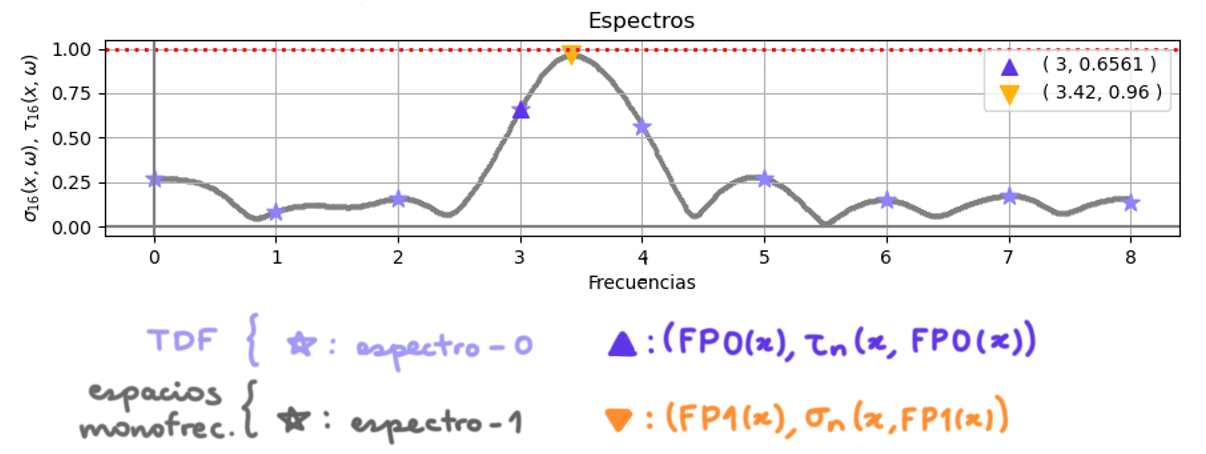
\includegraphics[scale = 1]{./estudios_espectrales/ejemplo_comparacion_1}
\end{figure}


Observe cómo el espectro-$1$ parece completar la información
dada por el espectro-$0$, pues, a diferencia del primero,
el espectro-$0$
da coeficientes de frecuencia $\tau_{n}(x, \omega)$ sólo
para algunas frecuencias enteras $\omega$, mientras que en el espectro-$1$
es posible considerar cualesquiera frecuencias $\omega \geq 0$; como puede observar
en la gráfica, 
\[
FP0 (x) = 3 \hspace{0.2cm} \textit{y} \hspace{0.2cm}
FP1 (x) = 3.42;
\]
esta segunda frecuencia es mucho más cercana a
la frecuencia real $\omega =3.4$ del sinusoide del que
fue obtenida la señal $x$; como agregamos ruido en las mediciones, no 
es de extrañarse que no se haya
obtenido exactamente $FP1(x) = 3.4$.

A pesar de que el espectro-$0$, el obtenido a partir de la
transformada discreta de Fourier, no dio una mala estimación (del rango
de frecuencias $Dom_{TDF,n}$ considerado por esta herramienta,
$\omega =3$ es el valor más cercano al valor real $\omega = 3.4$), vemos en este
ejemplo que usando el espectro-$1$ de una señal con una malla de
frecuencias $Dom_{\omega} \supseteq Dom_{TDF,n}$
suficientemente densa, es posible obtener mejores
estimaciones de frecuencias que modelen a la señal original. \\

Mostramos ahora la gráfica de $x$ junto con
\begin{itemize}
	\item la parte de la síntesis de $x$ respecto a la $TDF$
	que corresponde a la frecuencia principal
	$FP0(x)$ (c.f.
	nota \ref{nota: ya?}), que de hecho,
	según la nota \ref{nota: proyeciones monof TDF}, es
	$\Pi_{P_{36,3}}(x)$
	\begin{figure}[H]
			\sidecaption{
			Puesto que $\{ c_{36, 3}, s_{36, \omega} \}$
			es una BON de $P_{36, 3}$, claro que la señal 
			que resulta de discretizar el sinusoide morado en la malla
			$I_{36}$ es, de hecho, la proyección de $x$ 
			al espacio monofrecuencial $P_{36, 3}$.
 			\label{fig: comparacion 2}
			}
			\centering
			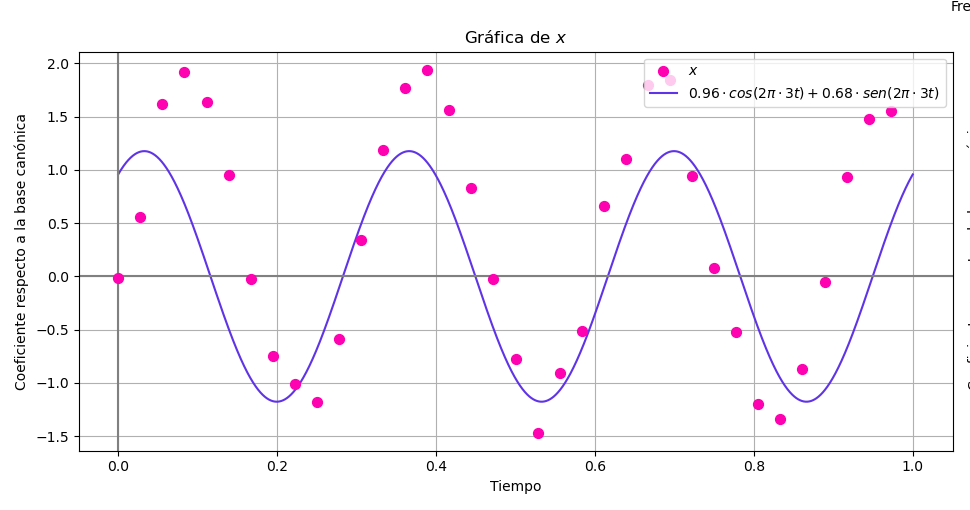
\includegraphics[scale = 0.5]{./estudios_espectrales/ejemplo_comparacion_2} 
		\end{figure}		
	
	y
	\item la señal $\Pi_{P_{16, 3.39}}(x)$, o sea, la señal de
	dimensión $16$ y frecuencia $FP1(x)=3.39$ más cercana a $x$, junto con
	el sinusoide continuo del que fue muestreado.
	\begin{figure}[H]
			\sidecaption{
			Para obtener la versión continua del sinusoide 
			discreto $\Pi_{P_{36, 3.42}}(x)$ (i.e. la gráfica naranja),
			usamos las fórmulas establecidas en los teoremas
			\ref{teo: amelie1} y \ref{teo: amelie2}.
			\label{fig: comparacion 3}
			}
			\centering
			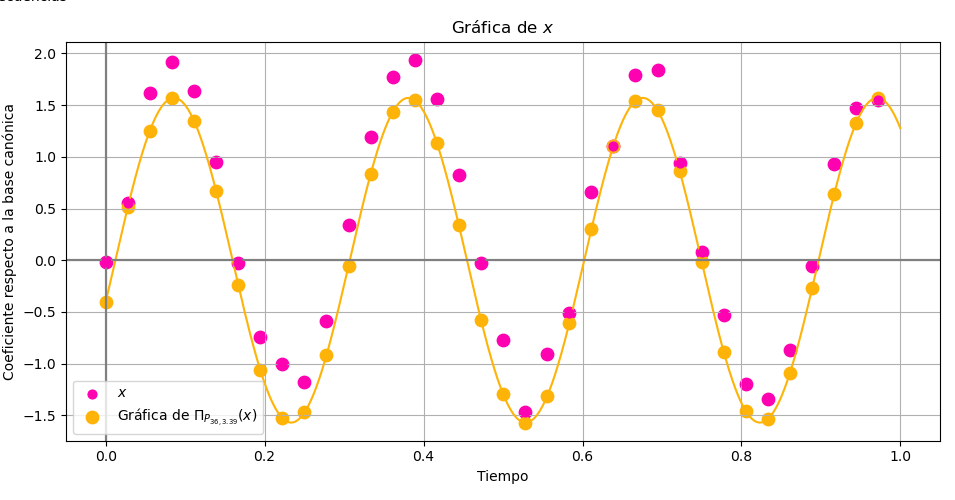
\includegraphics[scale = 0.5]{./estudios_espectrales/ejemplo_comparacion_3} 
		\end{figure}		
\end{itemize}


Los sinusoides de las figuras \ref{fig: comparacion 2} y
\ref{fig: comparacion 3}
son las señales de frecuencia pura
$3$ y $3.42$, respectivamente, cuya distancia euclidea
a la señal original $x$ es mínima. Observe que la segunda
señal, aquella cuya frecuencia
fue determinada
a partir del estudio espectral basado en espacios
monofrecuenciales,
parece ajustarse un poco mejor a la gráfica de $x$. \\

\begin{figure}[H]
			\sidecaption{
			Mostramos ahora los espectros de la señal $x$ que se obtiene
			tomando $36$ muestras uniformemente espaciadas del mismo sinusoide
			$f(t)$ de antes, esta vez sin agregar ruido aleatorio a las mediciones.
			Observe que el espectro-1 detectó a la frecuencia $\omega = 3.4$
			como la mejor, y que el sinusoide naranja ajusta perfectamente la gráfica
			de $x$. Como la frecuencia real no es entera, usando la frecuencia principal
			dada por la TDF sigue sin dar resultados perfectos, aunque no malos.
			\label{fig: sinusoide sin ruido}
			}
			\centering
			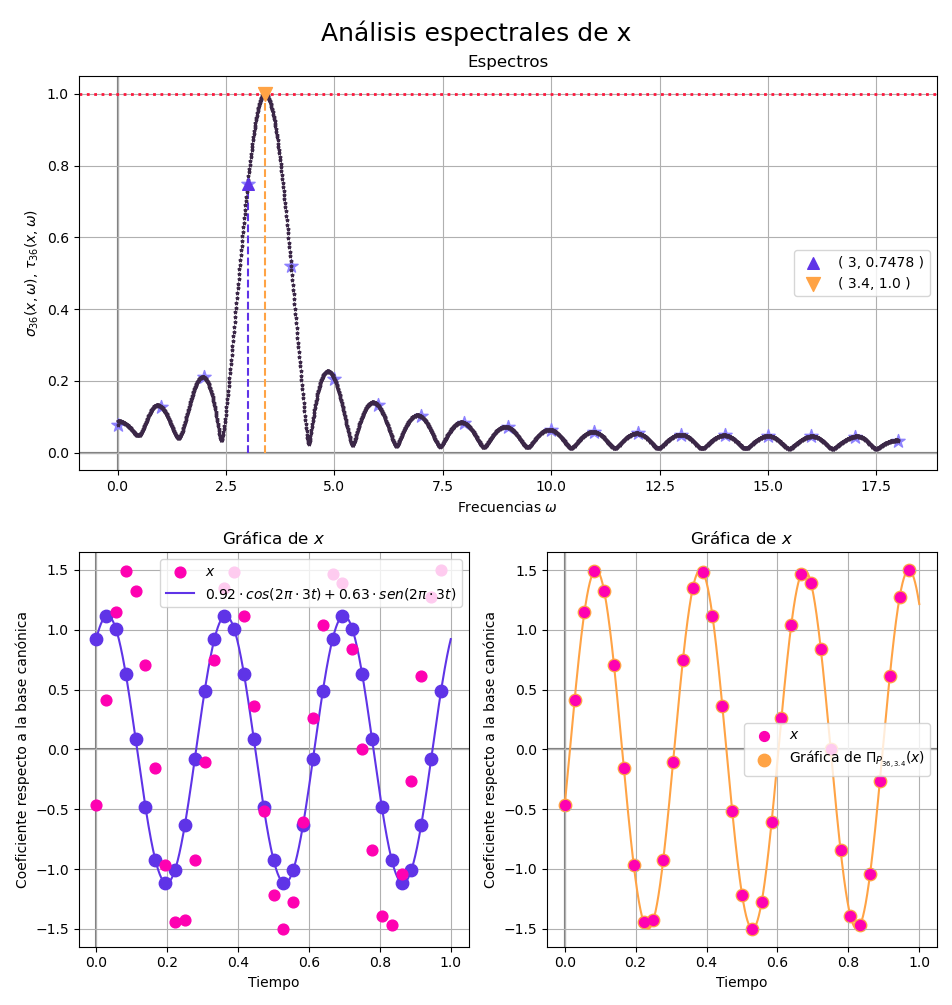
\includegraphics[scale = 0.4]{./estudios_espectrales/sinusoide_sin_ruido} 
		\end{figure}		

	\begin{figure}[H]
			\sidecaption{
			Si cambiamos la frecuencia dle sinusoide $f$ de este ejemplo
			a $\omega = 5$, como 
			era de esperarse, la frecuencia principal de ambos
			espectros es $5$
			(y el valor de los 
			espectros en tal frecuencia
			es igual a $1$, la cota
			superior). Además, 
			las gráficas de frecuencia $5$ que resultan
			ajustan a la perfección a la señal original $x$.
			\label{fig: comparacion 4}
			}
			\centering
			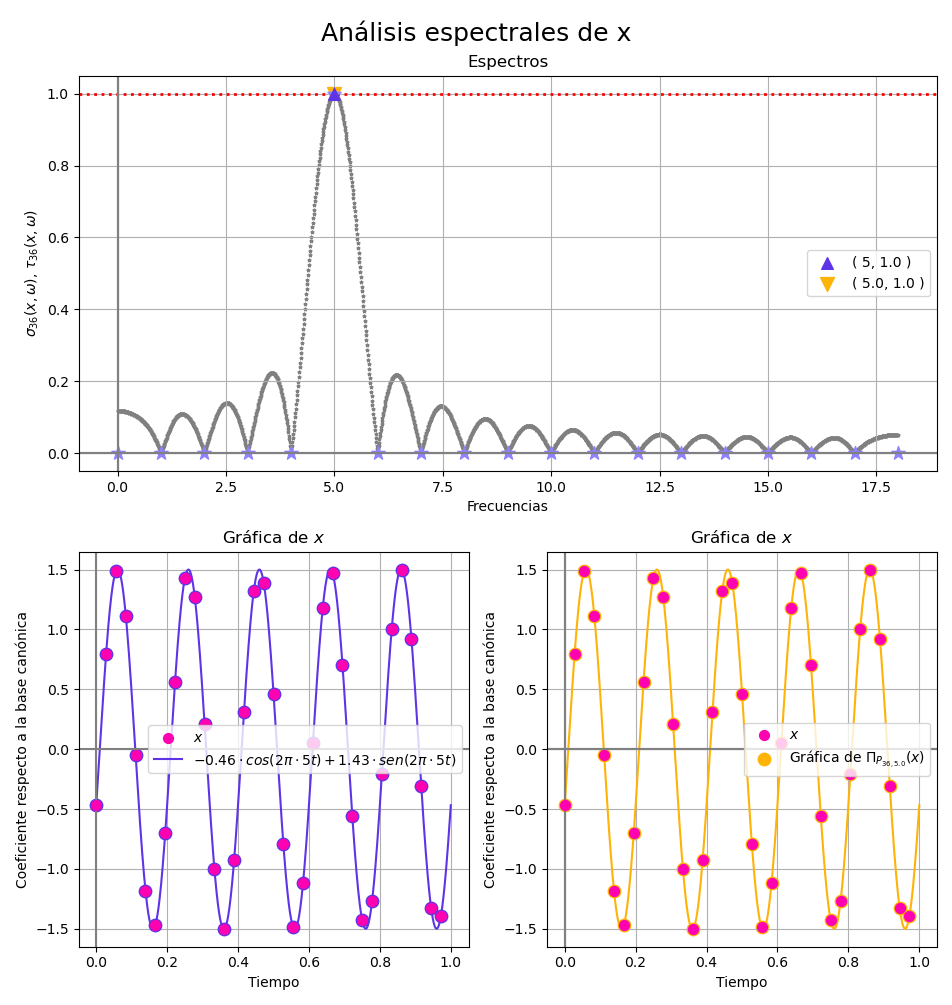
\includegraphics[scale = 0.4]{./estudios_espectrales/ejemplo_comparacion_4} 
		\end{figure}	

\final
\end{ejemplo}

\begin{nota}
\label{nota: la mejor frecuencia}
Según lo discutido en esta sección, fijados $n \geq 2$
y $x \in \IR^{n}$, \textbf{entre más cercano a $1$ sea 
el coeficiente $\tau_{n}(x, \omega)$ o 
$\sigma_{n}(x, \omega)$, mejor es usar un sinusoide
de frecuencia $\omega$ para ajustar la gráfica de $x$}.
Esto porque, recuerde, entre más cercano a uno sea uno de
esos coeficientes, más cercana estará la señal $x$ a tener
la propiedad de ser una discretización de un sinusoide
de la respectiva frecuencia.
\end{nota}

\subsection{Simetría, periodicidad y continuidad del espectro}

Para terminar este capítulo, 
fijada una dimensión $n \geq 2$,
vamos a establecer algunos
resultados sobre la periodicidad del espectro
de cualquier señal $x$, la simetría de la gráfica
del espectro respecto a cualquier punto de la forma
$\frac{n}{2} \IZ$ y terminamos con algunos comentarios
sobre la continuidad de este.

\begin{prop}
\label{prop: periodicidad espectro}
\textbf{(Periodicidad del espectro)}
Sean $x \in \IR^{n}$, $0 \leq \omega \leq \frac{n}{2}$.
Para toda $K \in \IZ$,
\[
\sigma_{n}(x, \omega) = \sigma_{n}(x, \omega + Kn).
\]
\end{prop}
\noindent
\textbf{Demostración.}
Sólo observe que 
\begin{align*}
\tilde{c}_{n, \omega + Kn} = & \left( cos \left( 2 \pi
\left( \omega + Kn \right) \frac{m}{n} \right) \right)_{m=0}^{n-1} \\
= & \left( cos \left( 
2 \pi \omega \frac{m}{n} + 2 \pi K m
\right) \right)_{m=0}^{n-1} \\
= & \left( cos \left( 
2 \pi \omega \frac{m}{n}
\right) \right)_{m=0}^{n-1} = \tilde{c}_{n, \omega}
\end{align*}
y, similarmente, que 
\[
\tilde{s}_{n, \omega + Kn} = \tilde{s}_{n, \omega},
\]
luego, por definición de los espacios monofrecuenciales
(c.f. ecuación \ref{eq: espacio Pnw}),
\begin{align*}
P_{n, \omega + Kn} =
& span(\tilde{c}_{n, \omega + Kn}, \tilde{s}_{n, \omega + Kn}) \\
= & span(\tilde{c}_{n, \omega }, \tilde{s}_{n, \omega }) = P_{n, \omega};
\end{align*}
de esto se concluye, usando la definición
\ref{def: final de sigmas},
que 
\[
\sigma_{n}(x, \omega) = 
cos (\measuredangle(x, P_{n, \omega}))
= cos (\measuredangle(x, P_{n, \omega + Kn})) = 
\sigma_{n}(x, \omega + Kn).
\]
\QEDB
\vspace{0.2cm}

\begin{figure}[H]
	\sidecaption{
	Según la periodicidad establecida en la proposición 
	\ref{prop: periodicidad espectro}, basta calcular los
	coeficientes espectrales
	$\sigma_{n}(x, \omega)$ para frecuencias
	$0 \leq \omega \leq n$.
	\label{fig: periodicidad espectro}
	}
	\centering
	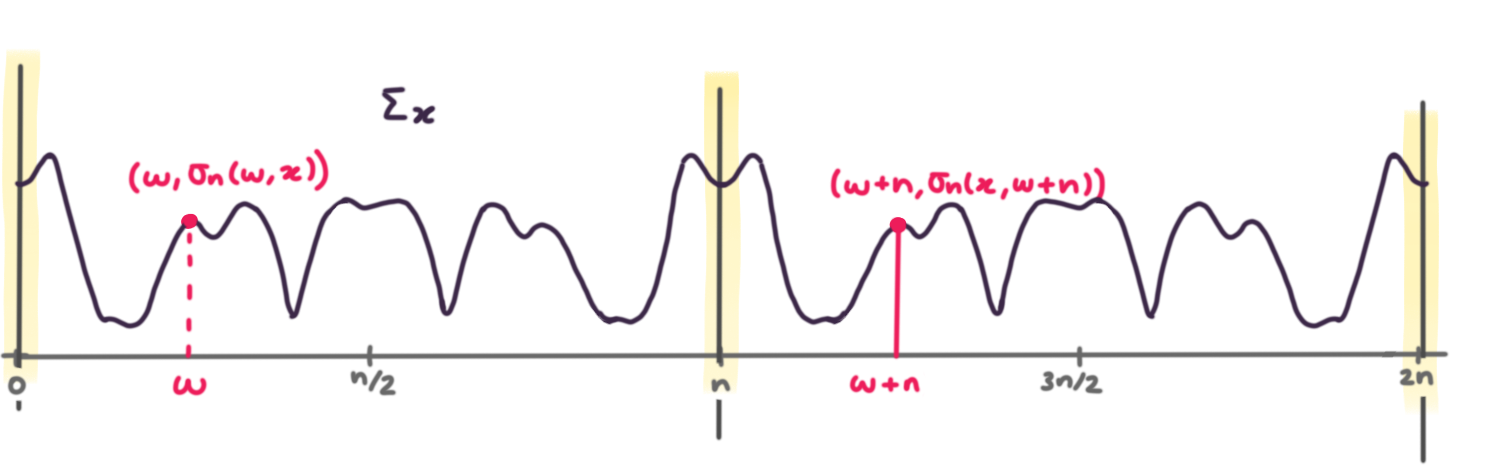
\includegraphics[scale = 0.9]{periodicidad_espectro} 
\end{figure}	


\begin{prop}
\textbf{(Simetría del espectro)}
Sean
$n \geq 2$,
$x \in \IR^{n}$. Para toda $0 \leq1 \omega \leq \frac{n}{2}$,
\[
\sigma_{n}(x, \omega) = 
\sigma_{n}(x, n-\omega ). 
\]
\end{prop}
\noindent
\textbf{Demostración.}
En efecto, 
\begin{align*}
\tilde{c}_{n, \omega + n} = & \left( cos \left( 2 \pi
\left( n- \omega \right) \frac{m}{n} \right) \right)_{m=0}^{n-1} \\
= & \left( cos \left( 
2 \pi n \frac{m}{n} - 2 \pi \omega
\frac{m}{n}
\right) \right)_{m=0}^{n-1} \\
= & \left( cos \left( 
2 \pi m - 2 \pi \omega \frac{m}{n} 
\right) \right)_{m=0}^{n-1} \\
= & \left( cos \left( 2 \pi \omega \frac{m}{n} \right) \right)_{m=0}^{n-1}
= \tilde{c}_{n, \omega}
\end{align*}
y, similarmente,
\[
\tilde{s}_{n, \omega + Kn} = -\tilde{s}_{n, \omega};
\]
de esto, como en la demostración de la proposición
\ref{prop: periodicidad espectro}, se concluye la igualdad
entre los espacios $P_{n, \omega}$ y $P_{n, n-\omega}$, y de esto
la igualdad deseada.
\QEDB
\vspace{0.2cm}

\begin{figure}[H]
	\sidecaption{
	Podemos así afinar la afirmación hecha en la figura 
	\ref{fig: periodicidad espectro} y concluir que basta
	calcular los coeficientes
	$\sigma_{n}(x, \omega)$ para $0 \leq \omega \leq \frac{n}{2}$,
	pues los demás pueden deducirse a partir de reflexiones y traslaciones.
	\label{fig: simetria espectro}
	}
	\centering
	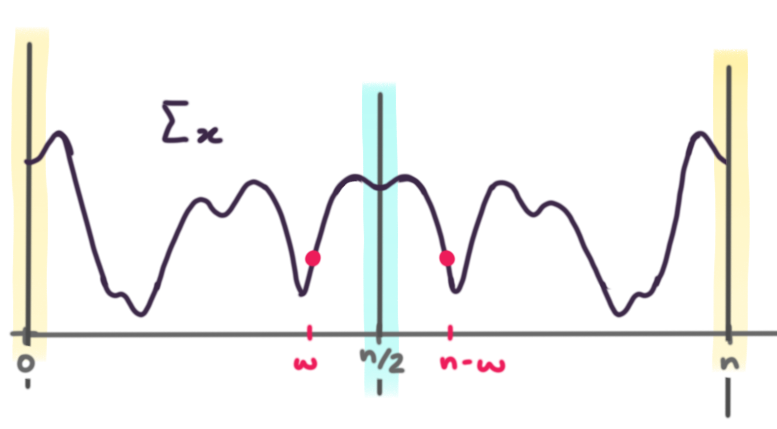
\includegraphics[scale = 1.4]{simetria_espectro} 
\end{figure}	


\TODO{Algunos comentarios sobre la continuidad y discontinuidad 
de salto del espectro en los puntos $\frac{n}{2}\IZ$.}